\documentclass{beamer}
\usetheme{metropolis}
\usepackage{graphicx}
\usepackage{subfig}
\title{Safe Return Doubtful: Week 5}
\date{\today}
\author{Jordan Hanson}
\institute{Whittier College Department of Physics and Astronomy}

\begin{document}
\maketitle

\section{Summary}

\begin{frame}{Summary}
\begin{enumerate}
\item Navigation in 3D: planning a hike to Rose Hills
\begin{itemize}
\item Using distance vectors
\item Accounting for elevation
\item Understanding \textit{power}
\item \textbf{Navigation with a compass}...calculating the distance to an object.
\end{itemize}
\item Radio-glaciology measurements
\begin{itemize}
\item Index of refraction, speed, distance, and time
\item Using exponentials, properties of exponentials
\item Attenuation length
\item Reflection coefficient
\end{itemize}
\end{enumerate}
\end{frame}

\section{Navigation in 3D}

\begin{frame}{Navigation in 3D}
We require several tools for navigation in 3D terrain.
\begin{itemize}
\item Review distance calculations in 2D (return to energy in a moment).
\item Altitude and energy, $W = mgh$.
\item Power: $P = E/t$.  Power is energy divided by time.
\item Establishing the distance to a far away object: triangulation.
\end{itemize}
\end{frame}

\begin{frame}{What is the horizontal distance to the water tower?}
\begin{figure}
\centering
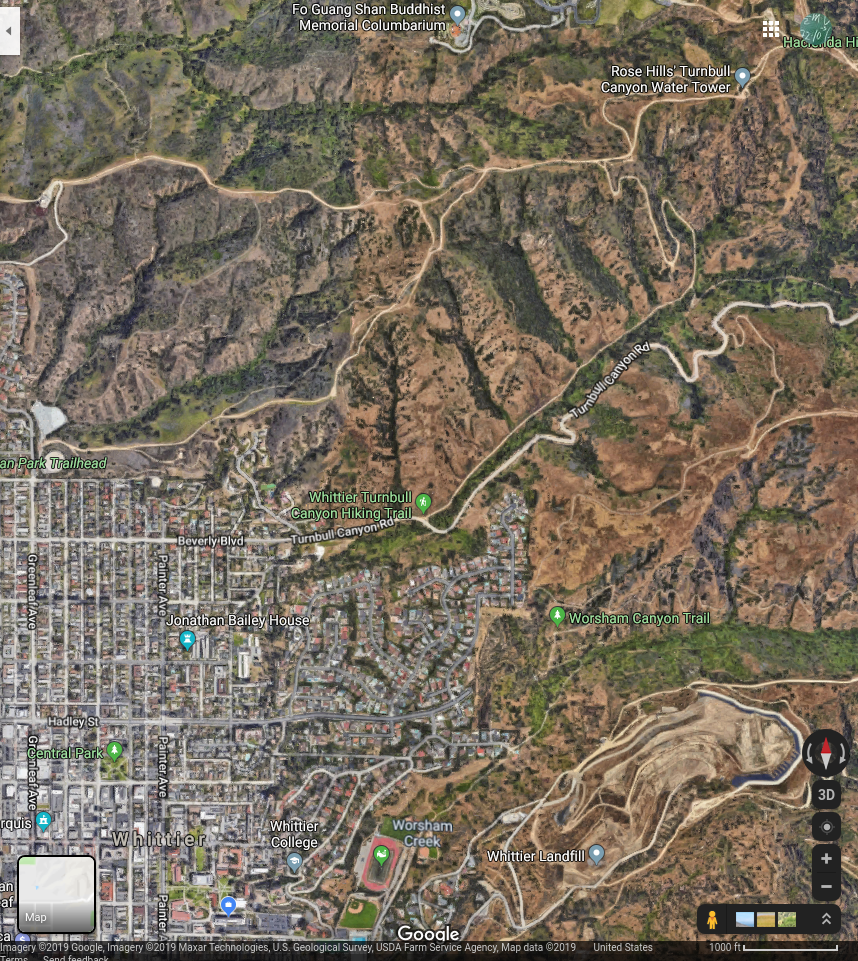
\includegraphics[width=0.55\textwidth]{areaMap.png}
\caption{\label{fig:area} A map including Whittier College and Turnbull Canyon.}
\end{figure}
\end{frame}

\begin{frame}{What energy is required to climb to some altitude?}
Energy required to ascend an altitude $h$:
\begin{equation}
W = m g h
\end{equation}
\begin{itemize}
\item $m$: mass in kilograms
\item $g$: 9.81 m/s$^2$
\item $h$: altitude in meters
\item $W$: energy in Joules
\end{itemize}
Assume the elevation above sea level of the water tower is 500 meters.  What energy is required?
\end{frame}

\begin{frame}{What power is required to climb to some altitude?}
Power is energy divided by time:
\begin{equation}
P = W/t
\end{equation}
\begin{itemize}
\item $P$: power in Watts (1 Joule/second)
\item $W$: energy in Joules
\item $t$: time in seconds
\end{itemize}
Assume the energy derived from the prior exercise.  Suppose the hike takes 2 hours.  What is the power consumption to make the climb?
\end{frame}

\begin{frame}{Correction: walking also requires power}
What power is required for walking?
\begin{figure}
\centering
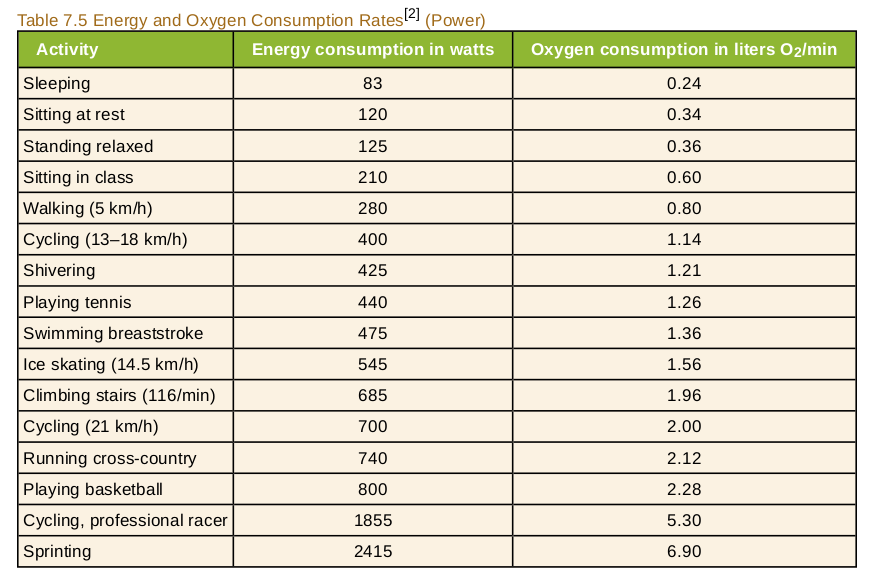
\includegraphics[width=0.7\textwidth]{powerTable.png}
\caption{\label{fig:power} Human activities and power consumption.}
\end{figure}
\end{frame}

\begin{frame}{What power is required to climb to some altitude?}
Power is energy divided by time:
\begin{equation}
P = W/t
\end{equation}
\begin{itemize}
\item $P$: power in Watts (1 Joule/second)
\item $W$: energy in Joules
\item $t$: time in seconds
\end{itemize}
\textbf{Now add the power consumption to the climbing exercise: what is the total power consumption?}
\end{frame}

\begin{frame}{Navigation with a compass: triangulation}
\begin{figure}
\centering
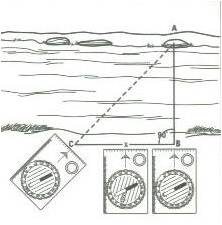
\includegraphics[width=0.5\textwidth]{Compass.jpg}
\caption{\label{fig:compass} The basic idea behind parallax and distance determination.}
\end{figure}
\end{frame}

\begin{frame}{Navigation with a compass: triangulation}
\begin{figure}
\centering
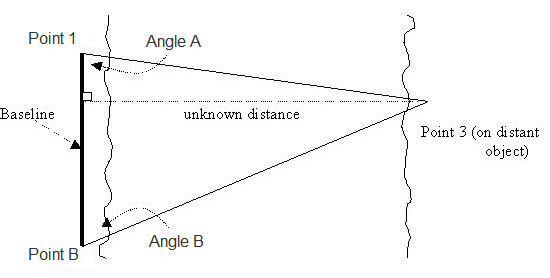
\includegraphics[width=0.65\textwidth]{triangle.png}
\caption{\label{fig:compass2} Using trigonometry to determine distance.}
\end{figure}
Let the unknown distance be called $d$.  Further, let the baseline be called $b = b_1 + b_2$.  We can show that
\begin{equation}
\boxed{
d = \left(\frac{\tan(A)\tan(B)}{\tan(A) + \tan(B)}\right)b}
\end{equation}
\end{frame}

\begin{frame}{Navigation with a compass: triangulation}
\small
\begin{equation}
\boxed{
d = \left(\frac{\tan(A)\tan(B)}{\tan(A) + \tan(B)}\right)b}
\end{equation}
Suppose we want the distance to a far away mountain.  We walk perpendicularly to the mountain after taking a compass \textit{bearing} that tells us $A = 70$ deg.  Our baseline is $b = 1000$ m.  We find $B = 60$ deg after taking a new bearing.  What is the distance $d$ to the object? \\ \vspace{1cm}
\textbf{Activity:}  What if we calculated the distance to Downtown LA by taking a bearing from Turnbull Canyon and the Science and Learning Center?
\end{frame}

\section{Radio-glaciology Measurements}

\begin{frame}{Radio-glaciology Measurements}
Index of refraction: the speed of radio waves is different in different materials.
\begin{equation}
v = \frac{c}{n}
\end{equation}
\begin{itemize}
\item $v$: Actual speed of radio wave in material
\item $c$: Speed of light, $3 \times 10^{8}$ m/s
\item $n$: A number close to 1
\end{itemize}
\end{frame}

\begin{frame}{Radio-glaciology Measurements}
\small
Attenuation length: the length over which the radio wave \textit{amplitude} decreases by a factor of $e$.
\begin{equation}
E = \frac{E_0}{r} \exp(-r/L)
\end{equation}
\begin{itemize}
\item $E$: Observed radio wave amplitude
\item $E_0$: Original radio wave amplitude
\item $r$: The total distance traveled
\item $L$: The \textit{attenuation length}.
\end{itemize}
\textbf{Observe example on board.}  Attenuation length varies with temperature.
\end{frame}

\section{Review of Attenuation Length of Ice}

\end{document}
